\subparagraph*{Submission : }
\textit{Do the same as Step 6 when the conversion rates are not stationary. Adopt a change-detection test approach.}\\

The goal is the same of the previous problem,but we have to manage the seasonality during the matching learning phase, using a change detection approach.

Implementation: \textit{n8.py}
\subsection*{Basic knowledge}
\subsubsection*{Change Detection (CUSUM)}
The first $M$ valid samples are used to produce the reference point.\\

Empirical mean of arm $a$ over the first $M$ valid samples $\bar{X_{a}^0}$\\

From the $M + 1-th$ valid sample on, we check whether there is a change\\

Positive deviation from the reference point at $t$ \hspace{0.2cm} $s_{a}^{+}(t) = (x_{a}(t) - \bar{X_{a}^0}(t)) - \epsilon$ \\

Negative deviation from the reference point at $t$ \hspace{0.2cm} $s_{a}^{-}(t) = -  (x_{a}(t) - \bar{X_{a}^0}(t)) - \epsilon$ \\

Cumulative positive deviation from the reference point at $t$ \hspace{0.2cm} $g_{a}^{+}(t) = \max \left\{0, g_{a}^{+}(t-1) + s_{a}^{+}(t) \right\}$ \\

Cumulative negative deviation from the reference point at $t$ \hspace{0.2cm} $g_{a}^{-}(t) = \max \left\{0, g_{a}^{-}(t-1) + s_{a}^{-}(t) \right\}$ \\

We have a change if \hspace{0.2cm} $g_{a}^{-}(t) > h$ or $g_{a}^{+}(t) > h$\\
\subsubsection*{CD-UCB} 
To the classical UCB algorithm is added a change detection mechanism. The bandit algorithm take the optimal decision, according with its past observation. During the update phase, the rewards are observed also by the change detection algorithm that monitos the distribution of each arms, and sends to the UCB a positive (or negative) signals in case of detection and the bandit reset the arm.

\underline{\textit{Pseudocode}}\\

1. Initialize $\tau_{a} = 0$ for $a\in A$ 

2. For each time $t$:\\

\hspace{0.8cm} $a_{t} \leftarrow \argmax_{a \in A}{\left\{\bar{x}_{a,\tau_{a},t} + \sqrt{\frac{2 log(n(t))}{{n_{a}(\tau_{a},t-1)}} }\right\}}$ with probability $1-\alpha$\\

\hspace{0.8cm} $a_{t} \leftarrow$ random arm with probability $1-\alpha$ \\

$n(t)$	is total number of valid samples\\

$\bar{x}_{a,\tau_{a},t}$ is the empirical mean of arm $a$ over the last valid samples\\

$n_{a}(\tau_{a},t-1)$ is the number of valid samples for arm $a$\\

3. Collect reward $r_t$\\

4. If $CD_a (r_{\tau},...,r_t) = 1$ then $\tau_a = t$ and restart $CD_a$

\subsubsection*{Promo-Category CD-UCB Matching} Also in this case we have developed a custom version of the UCB algorithm that we use in our scenarios. As for the modification we have done for the UCB without the change detection mechanism, we have added two matrices (support matrix and total reward matrix), used to compute the average reward obtained by each arm. The same initial phase of exploration (the starting delay) is adopted also in this case. The main difference is that we use a CD-UCB implementation and when a detection is present the two additional matrices are reset. 

\subsection*{Strategy}
In order to solve this problem we have used our customized implementation of Change Detection UCB algorithm, built on top of CUMSUM algorithm and classical UCB bandit algorithm. As for the previous submissions, we simulate the purchase of the two items client by client. We select the optimal superarm with the pricing learner, then, usign the Promo-Category CD-UCB we retrieve the optimal matching promotion-category for the current user. Finally we compute the rewards and update the learners. 

\subparagraph{Implementation}
\begin{itemize}
	\item Three seasons: Spring-Summer, Autumn, Winter
	\item Number of customers per class is not known 
	\item Candidates for the \textit{Racing Skis} are: \{2110.0, 1900.0, 2420.0, 2690.00\}
	\item Candidates for the \textit{Racing Ski Helmet} are: \{360.0, 410.0, 530.0, 600.0\}
	\item Conversion rate associated with the first item is not known
	\item Conversion rate associated with the second item is not known
	\item Promotion assignment is not known 
	\item Change-detection approach
\end{itemize} 

\subparagraph{Optimal strategy}
We have calculate the optimal solution in the same way as in step 7.\\
According to our candidates the optimal solution is:

\begin{center}
	\begin{tabular}{|c|p{4cm}|p{4cm}|p{4cm}|} 
		\hline
		Season & \textit{Racing Skis optimal price} & \textit{Racing Ski Helmet} optimal price & Optimal promo-category matching \\ \hline
		\multirow{4}{*}{Spring-Summer} & \multirow{4}{*}{1900.0} & \multirow{4}{*}{410.0} & Sport addicted: P$_0$ = 0\% (410.0)  \\ 
								   & 					   &                      & Gifted: P$_2$ = 20\% (328.0)          \\ 
								   & 					   &                      & Worried: P$_3$ = 30\% (287.0)         \\
								   & 					   &                      & Amateur: P$_1$ = 10\% (369.0)         \\ \hline
		\multirow{4}{*}{Autumn} & \multirow{4}{*}{2690.0} & \multirow{4}{*}{530.0}  & Sport addicted: P$_1$ = 10\% (477.0)\\ 
		& 					   &                      & Gifted: P$_3$ = 30\% (371.0)         \\ 
		& 					   &                      & Worried: P$_2$ = 20\% (424.0)         \\
		& 					   &                      & Amateur: P$_0$ = 0\% (530.0)         \\ \hline
		\multirow{4}{*}{Winter} & \multirow{4}{*}{2420.0} & \multirow{4}{*}{600.0}  & Sport addicted: P$_3$ = 30\% (420.0)\\ 
		& 					   &                      & Gifted: P$_1$ = 10\% (540.0)         \\ 
		& 					   &                      & Worried: P$_2$ = 20\% (480.0)         \\
		& 					   &                      & Amateur: P$_0$ = 0\% (600.0)          \\ \hline
	\end{tabular}
\end{center}

\subsection*{Results}
\begin{center}
	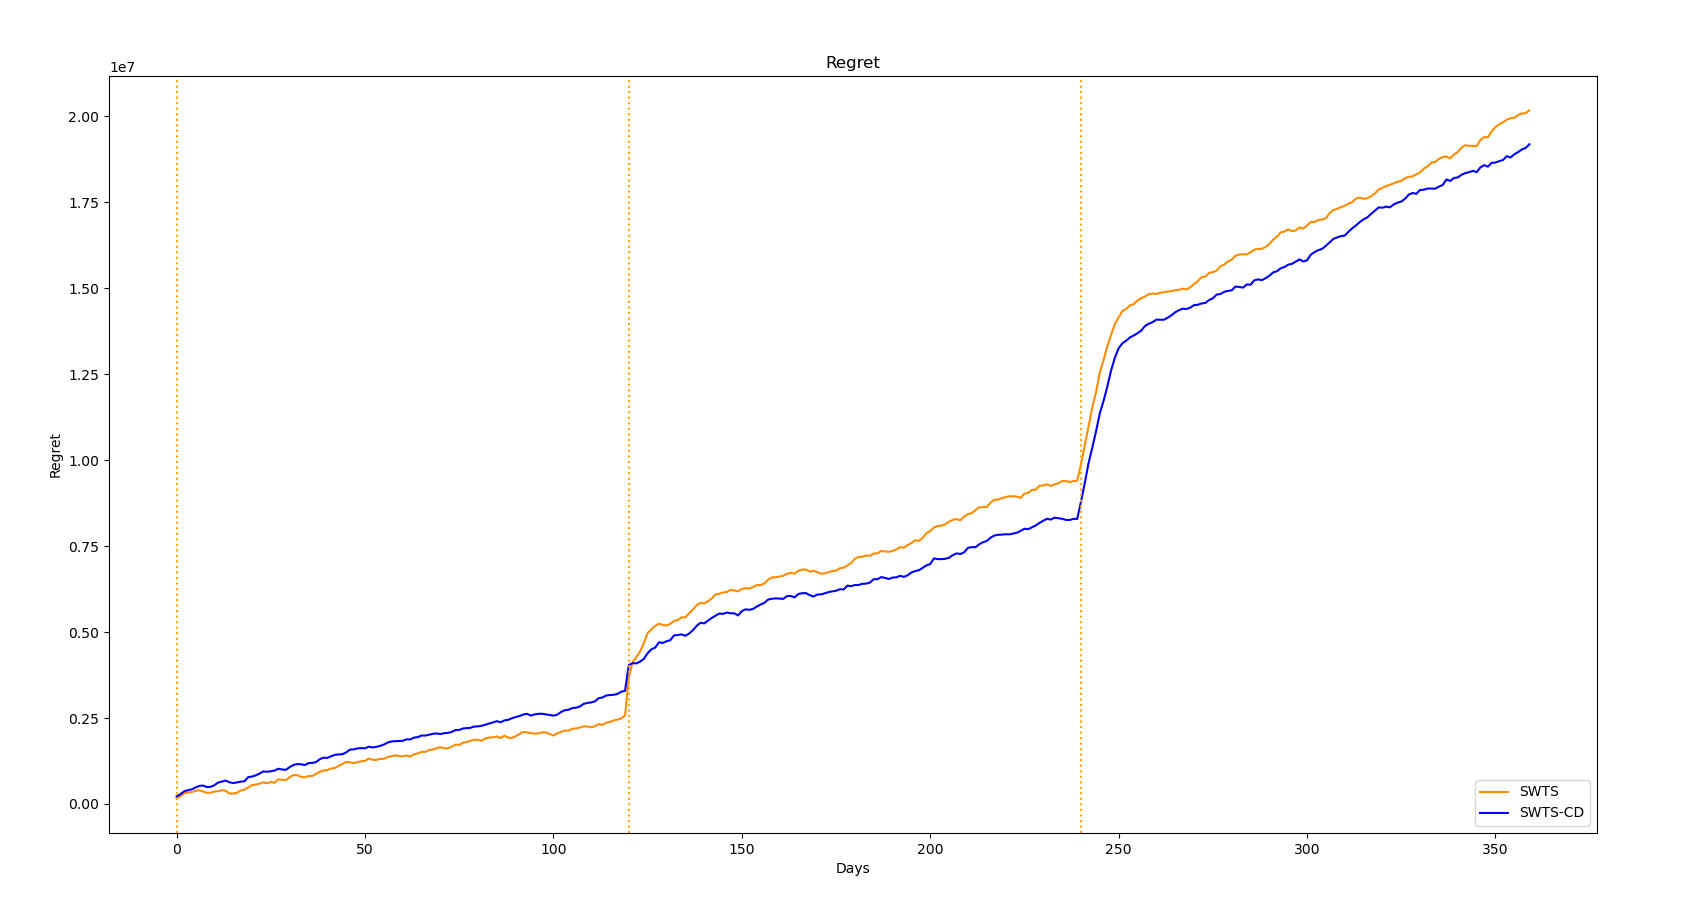
\includegraphics[scale=0.35]{Images/n8}
\end{center}

Days: 365\\
Experiments number: 2 \\
Season length : $|365/3| = 122 $ days\\
Starting delay of the Promo-Category CD-UCB Matching: 1000 clients\\
SWTS window size : $\sqrt{365 * 1000} * 30$\\

\subsection*{Considerations}
We can observe that the change detection approach has a smaller impact respect to the performance of the SWTS. This is due to the fact that the change detection approach catches some false positive detection; the matching of promo-category of the second item is influenced by the prices chosen for the two items.
